\documentclass[]{article}
\usepackage{lmodern}
\usepackage{amssymb,amsmath}
\usepackage{ifxetex,ifluatex}
\usepackage{fixltx2e} % provides \textsubscript
\ifnum 0\ifxetex 1\fi\ifluatex 1\fi=0 % if pdftex
  \usepackage[T1]{fontenc}
  \usepackage[utf8]{inputenc}
\else % if luatex or xelatex
  \ifxetex
    \usepackage{mathspec}
  \else
    \usepackage{fontspec}
  \fi
  \defaultfontfeatures{Ligatures=TeX,Scale=MatchLowercase}
\fi
% use upquote if available, for straight quotes in verbatim environments
\IfFileExists{upquote.sty}{\usepackage{upquote}}{}
% use microtype if available
\IfFileExists{microtype.sty}{%
\usepackage{microtype}
\UseMicrotypeSet[protrusion]{basicmath} % disable protrusion for tt fonts
}{}
\usepackage[margin=1in]{geometry}
\usepackage{hyperref}
\hypersetup{unicode=true,
            pdftitle={Data 612 Project 2 - Content-Based and Collaborative Filtering},
            pdfauthor={Vinayak Patel},
            pdfborder={0 0 0},
            breaklinks=true}
\urlstyle{same}  % don't use monospace font for urls
\usepackage{color}
\usepackage{fancyvrb}
\newcommand{\VerbBar}{|}
\newcommand{\VERB}{\Verb[commandchars=\\\{\}]}
\DefineVerbatimEnvironment{Highlighting}{Verbatim}{commandchars=\\\{\}}
% Add ',fontsize=\small' for more characters per line
\usepackage{framed}
\definecolor{shadecolor}{RGB}{248,248,248}
\newenvironment{Shaded}{\begin{snugshade}}{\end{snugshade}}
\newcommand{\AlertTok}[1]{\textcolor[rgb]{0.94,0.16,0.16}{#1}}
\newcommand{\AnnotationTok}[1]{\textcolor[rgb]{0.56,0.35,0.01}{\textbf{\textit{#1}}}}
\newcommand{\AttributeTok}[1]{\textcolor[rgb]{0.77,0.63,0.00}{#1}}
\newcommand{\BaseNTok}[1]{\textcolor[rgb]{0.00,0.00,0.81}{#1}}
\newcommand{\BuiltInTok}[1]{#1}
\newcommand{\CharTok}[1]{\textcolor[rgb]{0.31,0.60,0.02}{#1}}
\newcommand{\CommentTok}[1]{\textcolor[rgb]{0.56,0.35,0.01}{\textit{#1}}}
\newcommand{\CommentVarTok}[1]{\textcolor[rgb]{0.56,0.35,0.01}{\textbf{\textit{#1}}}}
\newcommand{\ConstantTok}[1]{\textcolor[rgb]{0.00,0.00,0.00}{#1}}
\newcommand{\ControlFlowTok}[1]{\textcolor[rgb]{0.13,0.29,0.53}{\textbf{#1}}}
\newcommand{\DataTypeTok}[1]{\textcolor[rgb]{0.13,0.29,0.53}{#1}}
\newcommand{\DecValTok}[1]{\textcolor[rgb]{0.00,0.00,0.81}{#1}}
\newcommand{\DocumentationTok}[1]{\textcolor[rgb]{0.56,0.35,0.01}{\textbf{\textit{#1}}}}
\newcommand{\ErrorTok}[1]{\textcolor[rgb]{0.64,0.00,0.00}{\textbf{#1}}}
\newcommand{\ExtensionTok}[1]{#1}
\newcommand{\FloatTok}[1]{\textcolor[rgb]{0.00,0.00,0.81}{#1}}
\newcommand{\FunctionTok}[1]{\textcolor[rgb]{0.00,0.00,0.00}{#1}}
\newcommand{\ImportTok}[1]{#1}
\newcommand{\InformationTok}[1]{\textcolor[rgb]{0.56,0.35,0.01}{\textbf{\textit{#1}}}}
\newcommand{\KeywordTok}[1]{\textcolor[rgb]{0.13,0.29,0.53}{\textbf{#1}}}
\newcommand{\NormalTok}[1]{#1}
\newcommand{\OperatorTok}[1]{\textcolor[rgb]{0.81,0.36,0.00}{\textbf{#1}}}
\newcommand{\OtherTok}[1]{\textcolor[rgb]{0.56,0.35,0.01}{#1}}
\newcommand{\PreprocessorTok}[1]{\textcolor[rgb]{0.56,0.35,0.01}{\textit{#1}}}
\newcommand{\RegionMarkerTok}[1]{#1}
\newcommand{\SpecialCharTok}[1]{\textcolor[rgb]{0.00,0.00,0.00}{#1}}
\newcommand{\SpecialStringTok}[1]{\textcolor[rgb]{0.31,0.60,0.02}{#1}}
\newcommand{\StringTok}[1]{\textcolor[rgb]{0.31,0.60,0.02}{#1}}
\newcommand{\VariableTok}[1]{\textcolor[rgb]{0.00,0.00,0.00}{#1}}
\newcommand{\VerbatimStringTok}[1]{\textcolor[rgb]{0.31,0.60,0.02}{#1}}
\newcommand{\WarningTok}[1]{\textcolor[rgb]{0.56,0.35,0.01}{\textbf{\textit{#1}}}}
\usepackage{graphicx}
% grffile has become a legacy package: https://ctan.org/pkg/grffile
\IfFileExists{grffile.sty}{%
\usepackage{grffile}
}{}
\makeatletter
\def\maxwidth{\ifdim\Gin@nat@width>\linewidth\linewidth\else\Gin@nat@width\fi}
\def\maxheight{\ifdim\Gin@nat@height>\textheight\textheight\else\Gin@nat@height\fi}
\makeatother
% Scale images if necessary, so that they will not overflow the page
% margins by default, and it is still possible to overwrite the defaults
% using explicit options in \includegraphics[width, height, ...]{}
\setkeys{Gin}{width=\maxwidth,height=\maxheight,keepaspectratio}
\IfFileExists{parskip.sty}{%
\usepackage{parskip}
}{% else
\setlength{\parindent}{0pt}
\setlength{\parskip}{6pt plus 2pt minus 1pt}
}
\setlength{\emergencystretch}{3em}  % prevent overfull lines
\providecommand{\tightlist}{%
  \setlength{\itemsep}{0pt}\setlength{\parskip}{0pt}}
\setcounter{secnumdepth}{0}
% Redefines (sub)paragraphs to behave more like sections
\ifx\paragraph\undefined\else
\let\oldparagraph\paragraph
\renewcommand{\paragraph}[1]{\oldparagraph{#1}\mbox{}}
\fi
\ifx\subparagraph\undefined\else
\let\oldsubparagraph\subparagraph
\renewcommand{\subparagraph}[1]{\oldsubparagraph{#1}\mbox{}}
\fi

%%% Use protect on footnotes to avoid problems with footnotes in titles
\let\rmarkdownfootnote\footnote%
\def\footnote{\protect\rmarkdownfootnote}

%%% Change title format to be more compact
\usepackage{titling}

% Create subtitle command for use in maketitle
\providecommand{\subtitle}[1]{
  \posttitle{
    \begin{center}\large#1\end{center}
    }
}

\setlength{\droptitle}{-2em}

  \title{Data 612 Project 2 - Content-Based and Collaborative Filtering}
    \pretitle{\vspace{\droptitle}\centering\huge}
  \posttitle{\par}
    \author{Vinayak Patel}
    \preauthor{\centering\large\emph}
  \postauthor{\par}
      \predate{\centering\large\emph}
  \postdate{\par}
    \date{2020-06-18}

\usepackage{booktabs}
\usepackage{longtable}
\usepackage{array}
\usepackage{multirow}
\usepackage{wrapfig}
\usepackage{float}
\usepackage{colortbl}
\usepackage{pdflscape}
\usepackage{tabu}
\usepackage{threeparttable}
\usepackage{threeparttablex}
\usepackage[normalem]{ulem}
\usepackage{makecell}
\usepackage{xcolor}

\begin{document}
\maketitle

\begin{Shaded}
\begin{Highlighting}[]
\ControlFlowTok{if}\NormalTok{ (}\OperatorTok{!}\KeywordTok{require}\NormalTok{(}\StringTok{"knitr"}\NormalTok{)) }\KeywordTok{install.packages}\NormalTok{(}\StringTok{"knitr"}\NormalTok{)}
\ControlFlowTok{if}\NormalTok{ (}\OperatorTok{!}\KeywordTok{require}\NormalTok{(}\StringTok{"tidyverse"}\NormalTok{)) }\KeywordTok{install.packages}\NormalTok{(}\StringTok{"tidyverse"}\NormalTok{)}
\ControlFlowTok{if}\NormalTok{ (}\OperatorTok{!}\KeywordTok{require}\NormalTok{(}\StringTok{"kableExtra"}\NormalTok{)) }\KeywordTok{install.packages}\NormalTok{(}\StringTok{"kableExtra"}\NormalTok{)}
\ControlFlowTok{if}\NormalTok{ (}\OperatorTok{!}\KeywordTok{require}\NormalTok{(}\StringTok{"dplyr"}\NormalTok{)) }\KeywordTok{install.packages}\NormalTok{(}\StringTok{"dplyr"}\NormalTok{)}
\ControlFlowTok{if}\NormalTok{ (}\OperatorTok{!}\KeywordTok{require}\NormalTok{(}\StringTok{"Matrix"}\NormalTok{)) }\KeywordTok{install.packages}\NormalTok{(}\StringTok{"Matrix"}\NormalTok{)}
\ControlFlowTok{if}\NormalTok{ (}\OperatorTok{!}\KeywordTok{require}\NormalTok{(}\StringTok{"recommenderlab"}\NormalTok{)) }\KeywordTok{install.packages}\NormalTok{(}\StringTok{"recommenderlab"}\NormalTok{)}
\ControlFlowTok{if}\NormalTok{ (}\OperatorTok{!}\KeywordTok{require}\NormalTok{(}\StringTok{"gridExtra"}\NormalTok{)) }\KeywordTok{install.packages}\NormalTok{(}\StringTok{"gridExtra"}\NormalTok{)}
\ControlFlowTok{if}\NormalTok{ (}\OperatorTok{!}\KeywordTok{require}\NormalTok{(}\StringTok{"graphics"}\NormalTok{)) }\KeywordTok{install.packages}\NormalTok{(}\StringTok{"graphics"}\NormalTok{)}
\end{Highlighting}
\end{Shaded}

~

\hypertarget{introduction}{%
\subsection{Introduction}\label{introduction}}

\textbf{For assignment 2, start with an existing dataset of user-item
ratings, such as our toy books dataset, MovieLens, Jester
{[}\url{http://eigentaste.berkeley.edu/dataset/}{]} or another dataset
of your choosing. Implement at least two of these recommendation
algorithms:}

{ • Content-Based Filtering • User-User Collaborative Filtering •
Item-Item Collaborative Filtering }

\textbf{As an example of implementing a Content-Based recommender, you
could build item profiles for a subset of MovieLens movies from scraping
\url{http://www.imdb.com/} or using the API at
\url{https://www.omdbapi.com/} (which has very recently instituted a
small monthly fee). A more challenging method would be to pull movie
summaries or reviews and apply tf-idf and/or topic modeling.}

{ You should evaluate and compare different approaches, using different
algorithms, normalization techniques, similarity methods, neighborhood
sizes, etc. You don't need to be exhaustive---these are just some
suggested possibilities.}

{ You may use the course text's recommenderlab or any other library that
you want.}

\hypertarget{data}{%
\subsection{Data}\label{data}}

\textbf{Load your data into (for example)} { } { I use MovieLens small
datasets: 100,000 ratings and 3,600 tag applications applied to 9,000
movies by 600 users. }

\begin{Shaded}
\begin{Highlighting}[]
\NormalTok{ratings_data <-}\StringTok{ }\KeywordTok{read.csv}\NormalTok{(}\StringTok{'ratings.csv'}\NormalTok{, }\DataTypeTok{stringsAsFactors =}\NormalTok{ F)}
\NormalTok{movie_data <-}\StringTok{ }\KeywordTok{read.csv}\NormalTok{(}\StringTok{'movies.csv'}\NormalTok{, }\DataTypeTok{stringsAsFactors =}\NormalTok{ F)}
\end{Highlighting}
\end{Shaded}

\begin{Shaded}
\begin{Highlighting}[]
\CommentTok{#Load results}
\KeywordTok{head}\NormalTok{(ratings_data) }\OperatorTok\StringTok{ }\KeywordTok{kable}\NormalTok{()}\OperatorTok
\StringTok{  }\KeywordTok{kable_styling}\NormalTok{(}\DataTypeTok{bootstrap_options =} \StringTok{"striped"}\NormalTok{, }\DataTypeTok{full_width =}\NormalTok{ F)}
\end{Highlighting}
\end{Shaded}

\begin{table}[H]
\centering
\begin{tabular}{r|r|r|r}
\hline
userId & movieId & rating & timestamp\\
\hline
1 & 1 & 4 & 964982703\\
\hline
1 & 3 & 4 & 964981247\\
\hline
1 & 6 & 4 & 964982224\\
\hline
1 & 47 & 5 & 964983815\\
\hline
1 & 50 & 5 & 964982931\\
\hline
1 & 70 & 3 & 964982400\\
\hline
\end{tabular}
\end{table}

\begin{Shaded}
\begin{Highlighting}[]
\KeywordTok{head}\NormalTok{(movie_data)}\OperatorTok\StringTok{ }\KeywordTok{kable}\NormalTok{()}\OperatorTok
\StringTok{  }\KeywordTok{kable_styling}\NormalTok{(}\DataTypeTok{bootstrap_options =} \StringTok{"striped"}\NormalTok{, }\DataTypeTok{full_width =}\NormalTok{ F)}
\end{Highlighting}
\end{Shaded}

\begin{table}[H]
\centering
\begin{tabular}{r|l|l}
\hline
movieId & title & genres\\
\hline
1 & Toy Story (1995) & Adventure|Animation|Children|Comedy|Fantasy\\
\hline
2 & Jumanji (1995) & Adventure|Children|Fantasy\\
\hline
3 & Grumpier Old Men (1995) & Comedy|Romance\\
\hline
4 & Waiting to Exhale (1995) & Comedy|Drama|Romance\\
\hline
5 & Father of the Bride Part II (1995) & Comedy\\
\hline
6 & Heat (1995) & Action|Crime|Thriller\\
\hline
\end{tabular}
\end{table}

\begin{Shaded}
\begin{Highlighting}[]
\CommentTok{### Structure}
\KeywordTok{str}\NormalTok{(ratings_data)}
\end{Highlighting}
\end{Shaded}

\begin{verbatim}
## 'data.frame':    100836 obs. of  4 variables:
##  $ userId   : int  1 1 1 1 1 1 1 1 1 1 ...
##  $ movieId  : int  1 3 6 47 50 70 101 110 151 157 ...
##  $ rating   : num  4 4 4 5 5 3 5 4 5 5 ...
##  $ timestamp: int  964982703 964981247 964982224 964983815 964982931 964982400 964980868 964982176 964984041 964984100 ...
\end{verbatim}

\begin{Shaded}
\begin{Highlighting}[]
\KeywordTok{str}\NormalTok{(movie_data)}
\end{Highlighting}
\end{Shaded}

\begin{verbatim}
## 'data.frame':    9742 obs. of  3 variables:
##  $ movieId: int  1 2 3 4 5 6 7 8 9 10 ...
##  $ title  : chr  "Toy Story (1995)" "Jumanji (1995)" "Grumpier Old Men (1995)" "Waiting to Exhale (1995)" ...
##  $ genres : chr  "Adventure|Animation|Children|Comedy|Fantasy" "Adventure|Children|Fantasy" "Comedy|Romance" "Comedy|Drama|Romance" ...
\end{verbatim}

\begin{Shaded}
\begin{Highlighting}[]
\CommentTok{### Summary}
\KeywordTok{str}\NormalTok{(movie_data)}
\end{Highlighting}
\end{Shaded}

\begin{verbatim}
## 'data.frame':    9742 obs. of  3 variables:
##  $ movieId: int  1 2 3 4 5 6 7 8 9 10 ...
##  $ title  : chr  "Toy Story (1995)" "Jumanji (1995)" "Grumpier Old Men (1995)" "Waiting to Exhale (1995)" ...
##  $ genres : chr  "Adventure|Animation|Children|Comedy|Fantasy" "Adventure|Children|Fantasy" "Comedy|Romance" "Comedy|Drama|Romance" ...
\end{verbatim}

\begin{Shaded}
\begin{Highlighting}[]
\KeywordTok{summary}\NormalTok{(movie_data)}
\end{Highlighting}
\end{Shaded}

\begin{verbatim}
##     movieId          title              genres         
##  Min.   :     1   Length:9742        Length:9742       
##  1st Qu.:  3248   Class :character   Class :character  
##  Median :  7300   Mode  :character   Mode  :character  
##  Mean   : 42200                                        
##  3rd Qu.: 76232                                        
##  Max.   :193609
\end{verbatim}

\hypertarget{transform-data}{%
\subsection{Transform Data}\label{transform-data}}

I use \texttt{realRatingMatrix} to transform data on Matrix value .

\begin{Shaded}
\begin{Highlighting}[]
\CommentTok{#### use pivot_wider to make a user matrix}
\NormalTok{ratings_data}\OperatorTok{$}\NormalTok{userId <-}\StringTok{ }\KeywordTok{as.factor}\NormalTok{(ratings_data}\OperatorTok{$}\NormalTok{userId)}
\NormalTok{movie_data}\OperatorTok{$}\NormalTok{movieId <-}\StringTok{ }\KeywordTok{as.factor}\NormalTok{(movie_data}\OperatorTok{$}\NormalTok{movieId)}
\NormalTok{ratings_data<-}\KeywordTok{subset}\NormalTok{(ratings_data, }\DataTypeTok{select=}\OperatorTok{-}\NormalTok{timestamp)}

\NormalTok{UI <-}\StringTok{ }\KeywordTok{as}\NormalTok{(ratings_data, }\StringTok{"realRatingMatrix"}\NormalTok{)}
\KeywordTok{str}\NormalTok{(UI)}
\end{Highlighting}
\end{Shaded}

\begin{verbatim}
## Formal class 'realRatingMatrix' [package "recommenderlab"] with 2 slots
##   ..@ data     :Formal class 'dgCMatrix' [package "Matrix"] with 6 slots
##   .. .. ..@ i       : int [1:100836] 0 4 6 14 16 17 18 20 26 30 ...
##   .. .. ..@ p       : int [1:9725] 0 215 325 377 384 433 535 589 597 613 ...
##   .. .. ..@ Dim     : int [1:2] 610 9724
##   .. .. ..@ Dimnames:List of 2
##   .. .. .. ..$ : chr [1:610] "1" "2" "3" "4" ...
##   .. .. .. ..$ : chr [1:9724] "1" "2" "3" "4" ...
##   .. .. ..@ x       : num [1:100836] 4 4 4.5 2.5 4.5 3.5 4 3.5 3 5 ...
##   .. .. ..@ factors : list()
##   ..@ normalize: NULL
\end{verbatim}

\begin{Shaded}
\begin{Highlighting}[]
\KeywordTok{dim}\NormalTok{(UI}\OperatorTok{@}\NormalTok{data)}
\end{Highlighting}
\end{Shaded}

\begin{verbatim}
## [1]  610 9724
\end{verbatim}

\#Users

\begin{Shaded}
\begin{Highlighting}[]
\CommentTok{#Users}
\NormalTok{similarity_users <-}\StringTok{ }\KeywordTok{similarity}\NormalTok{(UI[}\DecValTok{1}\OperatorTok{:}\DecValTok{10}\NormalTok{, ], }\DataTypeTok{method =} \StringTok{"cosine"}\NormalTok{, }\DataTypeTok{which =} \StringTok{"userId"}\NormalTok{)}

\CommentTok{# The more red the cell is, the more similar two users are. }
\KeywordTok{image}\NormalTok{(}\KeywordTok{as.matrix}\NormalTok{(similarity_users), }\DataTypeTok{main=}\StringTok{"User Similarity (cosine)"}\NormalTok{)}
\end{Highlighting}
\end{Shaded}

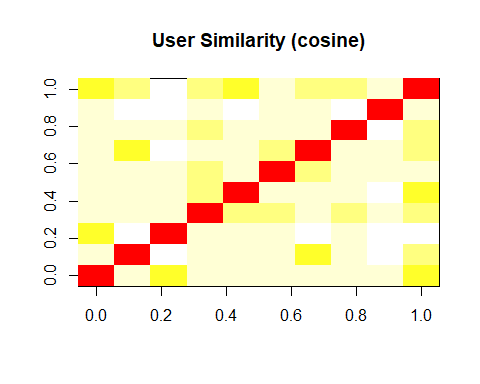
\includegraphics{Project_2_files/figure-latex/unnamed-chunk-6-1.pdf}
Items

\begin{Shaded}
\begin{Highlighting}[]
\CommentTok{#Items}
\NormalTok{similarity_items <-}\StringTok{ }\KeywordTok{similarity}\NormalTok{(UI[,}\DecValTok{1}\OperatorTok{:}\DecValTok{10}\NormalTok{], }\DataTypeTok{method =} \StringTok{"cosine"}\NormalTok{, }\DataTypeTok{which =} \StringTok{"items"}\NormalTok{)}
\CommentTok{# The more red the cell is, the more similar two users are. }
\KeywordTok{image}\NormalTok{(}\KeywordTok{as.matrix}\NormalTok{(similarity_items), }\DataTypeTok{main=}\StringTok{"Items Similarity (cosine)"}\NormalTok{)}
\end{Highlighting}
\end{Shaded}

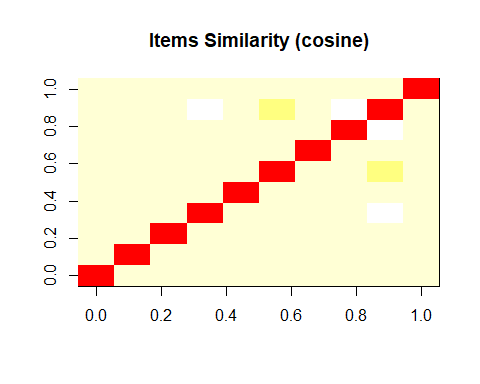
\includegraphics{Project_2_files/figure-latex/unnamed-chunk-7-1.pdf}

\hypertarget{split-training-and-test-datasets.}{%
\subsection{Split training and test
datasets.}\label{split-training-and-test-datasets.}}

I will make a matrix of ones and zeros which will facilitate extracting
the desired elements from the overall matrix.

\hypertarget{test-dataset}{%
\paragraph{Test dataset:}\label{test-dataset}}

\begin{Shaded}
\begin{Highlighting}[]
\CommentTok{### display UI_train}
\CommentTok{#UI_train %>% kable(caption = "TRAINING MATRIX")%>%}
\CommentTok{#  kable_styling(bootstrap_options = "striped", full_width = F)}

\CommentTok{### display UI_test}
\CommentTok{#UI_test %>% kable(caption = "TEST MATRIX")%>%}
\CommentTok{#  kable_styling(bootstrap_options = "striped", full_width = F)}
\end{Highlighting}
\end{Shaded}

\hypertarget{using-your-training-data-calculate-the-raw-average-mean-rating-for-every-user-item-combination.}{%
\subsection{Using your training data, calculate the raw average (mean)
rating for every user-item
combination.}\label{using-your-training-data-calculate-the-raw-average-mean-rating-for-every-user-item-combination.}}

\hypertarget{calculate-the-rmse-for-raw-average-for-both-your-training-data-and-your-test-data.}{%
\subsection{Calculate the RMSE for raw average for both your training
data and your test
data.}\label{calculate-the-rmse-for-raw-average-for-both-your-training-data-and-your-test-data.}}

\hypertarget{using-your-training-data-calculate-the-bias-for-each-user-and-each-item.}{%
\subsubsection{Using your training data, calculate the bias for each
user and each
item.}\label{using-your-training-data-calculate-the-bias-for-each-user-and-each-item.}}

\hypertarget{from-the-raw-average-and-the-appropriate-user-and-item-biases-calculate-the-baseline-predictors-for-every-user-item-combination.}{%
\subsubsection{From the raw average, and the appropriate user and item
biases, calculate the baseline predictors for every user-item
combination.}\label{from-the-raw-average-and-the-appropriate-user-and-item-biases-calculate-the-baseline-predictors-for-every-user-item-combination.}}

\hypertarget{calculate-the-rmse-for-the-baseline-predictors-for-both-your-training-data-and-your-test-data.}{%
\subsection{Calculate the RMSE for the baseline predictors for both your
training data and your test
data.}\label{calculate-the-rmse-for-the-baseline-predictors-for-both-your-training-data-and-your-test-data.}}

\hypertarget{summary-results.}{%
\subsection{Summary results.}\label{summary-results.}}

Lets calculate the percentage improvements based on the original (simple
average) and baseline predictor (including bias) RMSE numbers for both
Test and Train data sets.


\end{document}
